\documentclass{beamer}
\usepackage{etex}
\usepackage[utf8]{inputenc}
\usepackage[T1]{fontenc}
\usepackage{amssymb}
\usepackage{color}
\usepackage{verbatim}
\usepackage{beamerthemesplit}
\usepackage{graphicx}
\usepackage{xspace}
\usepackage{algorithm}
\usepackage{listings}
\usepackage{figlatex}
\usepackage{algorithmic}
\usepackage{multirow}

\graphicspath{{fig/}{campagne/fig}}
\newcommand{\talk}[2]{{#1} dit : {#2}}
\newcommand{\erik}[1]{\talk{Erik}{#1}}
\newcommand{\brice}[1]{\talk{Brice}{#1}}
\beamertemplatetransparentcovereddynamic

%\setbeamertemplate{background canvas}[vertical shading][bottom=red!10,top=blue!10]
%\usetheme{Warsaw}

\usecolortheme{progressbar}
\usefonttheme{progressbar}
\useoutertheme{progressbar}
\useinnertheme{progressbar}

\newcommand{\bordereau}{Bordereau\xspace}
\newcommand{\genepi}{Genepi\xspace}
\newcommand{\minelement}{{\em min\_element}\xspace}
\newcommand{\stablesort}{{\em stable\_sort}\xspace}
\newcommand{\merge}{{\em merge}\xspace}
\newcommand{\sort}{{\em sort}\xspace}
\newcommand{\find}{{\em find}\xspace}
\setbeamertemplate{navigation symbols}{}
\beamertemplatetransparentcovereddynamic
\newcommand{\pastel}{PaSTeL\xspace}

\definecolor{javared}{rgb}{0.6,0,0} % for strings
\definecolor{javagreen}{rgb}{0.30,0.55,0.40} % comments
\definecolor{javapurple}{rgb}{0.5,0,0.35} % keywords
\definecolor{javadocblue}{rgb}{0.25,0.35,0.75} % java


\title{BOAST}
\subtitle{Performance Portability Using Meta-Programming and Auto-Tuning}
\author[B. V.]{\textbf{Brice~Videau}~\inst{1}, Kevin~Pouget~\inst{1}, Luigi~Genovese~\inst{2},
                    Thierry~Deutsch~\inst{2}, Dimitri~Komatitsch~\inst{3}, Jean-François~Méhaut~\inst{1}}
\institute[INRIA]{\inst{1} INRIA - Corse, \inst{2} CEA - L\_Sim, \inst{3} CNRS}

\date{\textbf{Workshop JLESC}\\July 1, 2015}

\begin{document}

\frame{\titlepage}

\section{Introduction}

\subsection{Context}

\begin{frame}
  \frametitle{Scientific Application Portability}

  \begin{block}{\footnotesize Limited Portability}
    \begin{itemize}
      \item \scriptsize Huge codes (more than 100 000 lines), Written in FORTRAN or C++
      \item \scriptsize Collaborative efforts
      \item \scriptsize Use many different programing paradigms
    \end{itemize}
  \end{block}

  \begin{columns}

  \column{0.45\linewidth}
  \begin{block}{\footnotesize But Based on \emph{Computing Kernels}}
    \begin{itemize}
      \item \scriptsize Well defines part of a program
      \item \scriptsize Compute intensive
      \item \scriptsize Prime target for optimization
    \end{itemize}
  \end{block}

  \column{0.58\linewidth}
  \begin{block}{\footnotesize Kernels Should Be Written:}
    \begin{itemize}
      \item \scriptsize In a \emph{portable} manner
      \item \scriptsize In a way that raises developer \emph{productivity}
      \item \scriptsize To present good \emph{performance}
    \end{itemize}
  \end{block}

  \end{columns}

\end{frame}

\begin{frame}
  \frametitle{HPC Architecture Evolution}

  \begin{columns}

  \column{0.6\linewidth}
  \begin{block}{\footnotesize Very Rapid and Diverse, Top500:}
    \begin{itemize}
      \item \scriptsize Intel processor + Xeon Phi (Tianhe-2)
      \item \scriptsize AMD processor + nVidia GPU (Titan)
      \item \scriptsize IBM BlueGene/Q (Sequoia)
      \item \scriptsize Fujitsu SPARC64 (K Computer)
      \item \scriptsize Intel processor + nVidia GPU (Tianhe-1)
      \item \scriptsize AMD processor (Jaguar)
    \end{itemize}
  \end{block}

  \column{0.4\linewidth}
  \begin{block}{\footnotesize Tomorrow?}
    \begin{itemize}
      \item \scriptsize ARM + DSP?
      \item \scriptsize Intel Atom + FPGA?
      \item \scriptsize Quantum computing?
    \end{itemize}
  \end{block}

  \end{columns}

  \vspace{1cm}
  How to write kernels that could adapt to those architectures?\\
  (well maybe not quantum computing...)

\end{frame}

\section{A Parametrized Generator}

\begin{frame}

  \frametitle{Classical Tuning of Computing Kernels}

  \begin{center}%
    \includegraphics<1>[scale=1]{Workflow1-1}%
    \includegraphics<2>[scale=1]{Workflow1-2}%
    \includegraphics<3>[scale=1]{Workflow1-3}%
    \includegraphics<4>[scale=1]{Workflow1-4}%
  \end{center}%
  \begin{itemize}%
\only<1>{    \item Kernel optimization workflow}%
\only<1>{    \item Usually performed by a knowledgeable developer}%
\only<2>{    \item Compilers perform optimizations}%
\only<2>{    \item Architecture specific or generic optimizations}%
\only<3>{    \item Performance data hint at source transformations}%
\only<3>{    \item Architecture specific or generic hints}%
\only<4>{    \item Multiplication of kernel versions or loss of versions}%
\only<4>{    \item Difficulty to benchmark versions against each-other}%
  \end{itemize}%

\end{frame}

\begin{frame}
  \frametitle{BOAST Workflow \vphantom{Cp}}
  \begin{center}
    \includegraphics<1>[scale=1]{Workflow2-1}
    \includegraphics<2>[scale=1]{Workflow2-2}
    \includegraphics<3>[scale=1]{Workflow2-3}
  \end{center}
  \begin{itemize}%
\only<1>{    \item Meta-programming of optimizations in BOAST }
\only<1>{    \item High level object oriented language }
\only<2>{    \item Generate combination of optimizations }
\only<2>{    \item C, OpenCL, FORTRAN and CUDA are supported }
\only<3>{    \item Compilation and analysis are automated }
\only<3>{    \item Selection of best version can also be automated \vphantom{Cp}}
  \end{itemize}%
\end{frame}

\begin{frame}
\frametitle{BOAST Architecture}
 \begin{center}
   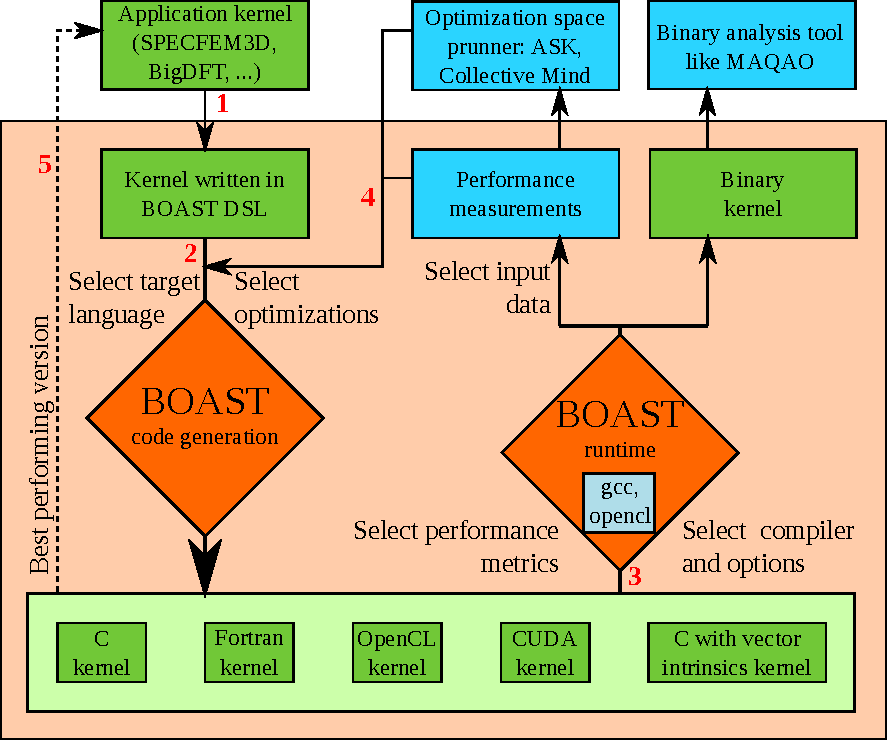
\includegraphics[scale=0.5]{BOAST_Workflow}
 \end{center}
\end{frame}

\section{Case Study}

\begin{frame}[fragile]
  \frametitle{Example: Laplace Kernel from ARM}
\tiny
\lstset{language=C,
basicstyle=\ttfamily,
keywordstyle=\color{javagreen}\bfseries,
stringstyle=\color{javared},
commentstyle=\color{javapurple},
numbers=left,
tabsize=4,
showspaces=false,
showstringspaces=false}
\begin{lstlisting}
void laplace(const int width,
             const int height,
             const unsigned char src[height][width][3],
                   unsigned char dst[height][width][3]){
  for (int j = 1; j < height-1; j++) {
    for (int i = 1; i < width-1; i++) {
      for (int c = 0; c < 3; c++) {
        int tmp = -src[j-1][i-1][c] -   src[j-1][i][c] - src[j-1][i+1][c]\
                 - src[j  ][i-1][c] + 9*src[j  ][i][c] - src[j  ][i+1][c]\
                 - src[j+1][i-1][c] -   src[j+1][i][c] - src[j+1][i+1][c];
        dst[j][i][c] = (tmp < 0 ? 0 : (tmp > 255 ? 255 : tmp));
      }
    }
  }
}
\end{lstlisting}
\begin{itemize}
\item C reference implementation
\item Many opportunities for improvement
\end{itemize}
\end{frame}

\begin{frame}[fragile]
  \frametitle{Example: Laplace in OpenCL}
\tiny
\lstset{language=C,
basicstyle=\ttfamily,
keywordstyle=\color{javagreen}\bfseries,
morekeywords={kernel,global,uchar},
stringstyle=\color{javared},
commentstyle=\color{javapurple},
numbers=left,
tabsize=4,
showspaces=false,
showstringspaces=false}
\begin{lstlisting}
kernel laplace(const int width,
               const int height,
               global const uchar *src,
               global       uchar *dst){
  int i = get_global_id(0);
  int j = get_global_id(1);
  for (int c = 0; c < 3; c++) {
    int tmp = -src[3*width*(j-1) + 3*(i-1) + c]\
             - src[3*width*(j-1) + 3*(i  ) + c]\
             - src[3*width*(j-1) + 3*(i+1) + c]\
             - src[3*width*(j  ) + 3*(i-1) + c]\
           + 9*src[3*width*(j  ) + 3*(i  ) + c]\
             - src[3*width*(j  ) + 3*(i+1) + c]\
             - src[3*width*(j+1) + 3*(i-1) + c]\
             - src[3*width*(j+1) + 3*(i  ) + c]\
             - src[3*width*(j+1) + 3*(i+1) + c];
    dst[3*width*j + 3*i + c] = clamp(tmp, 0, 255);
  }
}
\end{lstlisting}
\begin{itemize}
\item OpenCL reference implementation
\item Outer loops mapped to threads
\end{itemize}
\end{frame}

\begin{frame}[fragile]
  \frametitle{Example: Vectorizing}
\lstset{language=C,
basicstyle=\ttfamily,
keywordstyle=\color{javagreen}\bfseries,
morekeywords={kernel, global, uchar, uchar16, int16},
stringstyle=\color{javared},
commentstyle=\color{javapurple},
numbers=left,
tabsize=4,
showspaces=false,
showstringspaces=false}
\fontsize{3}{3}\selectfont
\begin{lstlisting}
kernel laplace(const int width,
               const int height,
               global const uchar *src,
               global       uchar *dst){
  int i = get_global_id(0);
  int j = get_global_id(1);
  uchar16 v11_ = vload16( 0, src + 3*width*(j-1) + 3*5*i - 3 );
  uchar16 v12_ = vload16( 0, src + 3*width*(j-1) + 3*5*i     );
  uchar16 v13_ = vload16( 0, src + 3*width*(j-1) + 3*5*i + 3 );
  uchar16 v21_ = vload16( 0, src + 3*width*(j  ) + 3*5*i - 3 );
  uchar16 v22_ = vload16( 0, src + 3*width*(j  ) + 3*5*i     );
  uchar16 v23_ = vload16( 0, src + 3*width*(j  ) + 3*5*i + 3 );
  uchar16 v31_ = vload16( 0, src + 3*width*(j+1) + 3*5*i - 3 );
  uchar16 v32_ = vload16( 0, src + 3*width*(j+1) + 3*5*i     );
  uchar16 v33_ = vload16( 0, src + 3*width*(j+1) + 3*5*i + 3 );
  int16 v11 = convert_int16(v11_);
  int16 v12 = convert_int16(v12_);
  int16 v13 = convert_int16(v13_);
  int16 v21 = convert_int16(v21_);
  int16 v22 = convert_int16(v22_);
  int16 v23 = convert_int16(v23_);
  int16 v31 = convert_int16(v31_);
  int16 v32 = convert_int16(v32_);
  int16 v33 = convert_int16(v33_);
  int16 res = v22 * (int)9 - v11 - v12 - v13 - v21 - v23 - v31 - v32 - v33;
        res = clamp(res, (int16)0, (int16)255);
  uchar16 res_ = convert_uchar16(res);
  vstore8(res_.s01234567, 0, dst + 3*width*j + 3*5*i);
  vstore8(res_.s89ab,     0, dst + 3*width*j + 3*5*i + 8);
  vstore8(res_.scd,       0, dst + 3*width*j + 3*5*i + 12);
  dst[3*width*j + 3*5*i + 14] = res_.se;
}
\end{lstlisting}
\begin{itemize}
\item Vectorized OpenCL implementation
\item 5 pixels (15 compoenets)
\end{itemize}
\end{frame}

\begin{frame}[fragile]
  \frametitle{Example: Synthesizing Vectors}
\lstset{language=C,
basicstyle=\ttfamily,
keywordstyle=\color{javagreen}\bfseries,
morekeywords={kernel, global, uchar, uchar16, int16},
stringstyle=\color{javared},
commentstyle=\color{javapurple},
numbers=left,
tabsize=4,
showspaces=false,
showstringspaces=false}
\tiny
\begin{lstlisting}
uchar16 v11_ = vload16( 0, src + 3*width*(j-1) + 3*5*i - 3 );
uchar16 v12_ = vload16( 0, src + 3*width*(j-1) + 3*5*i     );
uchar16 v13_ = vload16( 0, src + 3*width*(j-1) + 3*5*i + 3 );
uchar16 v21_ = vload16( 0, src + 3*width*(j  ) + 3*5*i - 3 );
uchar16 v22_ = vload16( 0, src + 3*width*(j  ) + 3*5*i     );
uchar16 v23_ = vload16( 0, src + 3*width*(j  ) + 3*5*i + 3 );
uchar16 v31_ = vload16( 0, src + 3*width*(j+1) + 3*5*i - 3 );
uchar16 v32_ = vload16( 0, src + 3*width*(j+1) + 3*5*i     );
uchar16 v33_ = vload16( 0, src + 3*width*(j+1) + 3*5*i + 3 );
\end{lstlisting}
\normalsize
\centering Becomes
\tiny
\begin{lstlisting}
uchar16 v11_ = vload16( 0, src + 3*width*(j-1) + 3*5*i - 3 );
uchar16 v13_ = vload16( 0, src + 3*width*(j-1) + 3*5*i + 3 );
uchar16 v12_ = uchar16( v11_.s3456789a, v13_.s56789abc );
uchar16 v21_ = vload16( 0, src + 3*width*(j  ) + 3*5*i - 3 );
uchar16 v23_ = vload16( 0, src + 3*width*(j  ) + 3*5*i + 3 );
uchar16 v22_ = uchar16( v21_.s3456789a, v23_.s56789abc );
uchar16 v31_ = vload16( 0, src + 3*width*(j+1) + 3*5*i - 3 );
uchar16 v33_ = vload16( 0, src + 3*width*(j+1) + 3*5*i + 3 );
uchar16 v32_ = uchar16( v31_.s3456789a, v33_.s56789abc );
\end{lstlisting}
\begin{itemize}
\item Synthesizing loads should save bandwidth
\item Could be pushed further
\end{itemize}
\end{frame}

\begin{frame}[fragile]
  \frametitle{Example: Reducing Variable Size}
\lstset{language=C,
basicstyle=\ttfamily,
keywordstyle=\color{javagreen}\bfseries,
morekeywords={kernel, global, uchar, uchar16, int16, short16},
stringstyle=\color{javared},
commentstyle=\color{javapurple},
numbers=left,
tabsize=4,
showspaces=false,
showstringspaces=false}
\tiny
\begin{lstlisting}
int16 v11 = convert_int16(v11_);
int16 v12 = convert_int16(v12_);
int16 v13 = convert_int16(v13_);
int16 v21 = convert_int16(v21_);
int16 v22 = convert_int16(v22_);
int16 v23 = convert_int16(v23_);
int16 v31 = convert_int16(v31_);
int16 v32 = convert_int16(v32_);
int16 v33 = convert_int16(v33_);
int16 res = v22 * (int)9 - v11 - v12 - v13 - v21 - v23 - v31 - v32 - v33;
      res = clamp(res, (int16)0, (int16)255);
\end{lstlisting}
\normalsize
\centering Becomes
\tiny
\begin{lstlisting}
short16 v11 = convert_short16(v11_);
short16 v12 = convert_short16(v12_);
short16 v13 = convert_short16(v13_);
short16 v21 = convert_short16(v21_);
short16 v22 = convert_short16(v22_);
short16 v23 = convert_short16(v23_);
short16 v31 = convert_short16(v31_);
short16 v32 = convert_short16(v32_);
short16 v33 = convert_short16(v33_);
short16 res = v22 * (short)9 - v11 - v12 - v13 - v21 - v23 - v31 - v32 - v33;
        res = clamp(res, (short16)0, (short16)255);
\end{lstlisting}
\begin{itemize}
\item Using smaller intermediary types could save registers
\end{itemize}
\end{frame}

\begin{frame}
  \frametitle{Example: Optimization Summary}
  \begin{itemize}
    \item Very complex process
    \item Intimate knowledge of the architecture required
    \item Numerous versions to be benchmarked
    \item Difficult to test combination of optimizations:
    \begin{itemize}
      \item Vectorization,
      \item Intermediary data type,
      \item Number of pixels processed,
      \item Synthesizing loads.
    \end{itemize}
    \item Can we use BOAST to automate the process?
  \end{itemize}
\end{frame}

\begin{frame}
  \frametitle{Example: Laplace Kernel with BOAST}
  \begin{itemize}
    \item Based on components instead of pixel
    \item Use tiles rather than only sequence of elements
    \item Parameters used in the BOAST version:
    \begin{itemize}
      \item \emph{x\_component\_number}: a positive integer
      \item \emph{y\_component\_number}: a positive integer
      \item \emph{vector\_length}: 1, 2, 4, 8 or 16
      \item \emph{temporary\_size}: 2 or 4
      \item \emph{synthesizing\_loads}: true or false
    \end{itemize}
  \end{itemize}
\end{frame}

\begin{frame}
  \frametitle{Example: ARM results}
  \begin{center}
  \scriptsize
  \begin{tabular}{c|r|r|c|r|c}
    Image Size  & Naive (s) & Best (s) & Acceleration & BOAST (s) & Acceleration \\
    \hline&&&&\\
  768 x 432   & 0.0107    & 0.00669  & x1.6         & 0.000639  & x16.7 \\
  2560 x 1600 & 0.0850    & 0.0137   & x6.2         & 0.00687   & x12.4 \\
  2048 x 2048 & 0.0865    & 0.0149   & x5.8         & 0.00715   & x12.1 \\
  5760 x 3240 & 0.382     & 0.0449   & x8.5         & 0.0325    & x11.8 \\
  7680 x 4320 & 0.680     & 0.0747   & x9.1         & 0.0581    & x11.7
  \end{tabular}
  \end{center}

  \begin{itemize}
    \item Optimal parameters values:
    \begin{itemize}
      \item x\_component\_number: 16
      \item y\_component\_number: 1
      \item vector\_length: 16
      \item temporary\_size: 2
      \item synthesizing\_loads: false
    \end{itemize}
    \item Close to what ARM engineers found
  \end{itemize}
\end{frame}

\begin{frame}
  \frametitle{Example: Performance Portability}
  \begin{center}
  \scriptsize
  \begin{tabular}{c|r|r|c|r|c}
    Image Size & BOAST ARM (s) & BOAST Intel & Ratio & BOAST NVIDIA & Ratio \\
    \hline&&&&\\
  768 x 432   & 0.000639     & 0.000222    & x2.9  & 0.0000715    & x8.9  \\
  2560 x 1600 & 0.00687      & 0.00222     & x3.1  & 0.000782     & x8.8  \\
  2048 x 2048 & 0.00715      & 0.00226     & x3.2  & 0.000799     & x8.9  \\
  5760 x 3240 & 0.0325       & 0.0108      & x3.0  & 0.00351      & x9.3  \\
  7680 x 4320 & 0.0581       & 0.0192      & x3.0  & 0.00623      & x9.3
  \end{tabular}
  \end{center}

  \begin{columns}
  \column{0.5\textwidth}

  \begin{itemize}
    \item \footnotesize Optimal parameters values Intel:
    \begin{itemize}
      \item \scriptsize x\_component\_number: 16
      \item \scriptsize y\_component\_number: 4..2
      \item \scriptsize vector\_length: 8
      \item \scriptsize temporary\_size: 2
      \item \scriptsize synthesizing\_loads: false
    \end{itemize}
  \end{itemize}
  \column{0.5\textwidth}
  \begin{itemize}
    \item \footnotesize Optimal parameters values NVIDIA:
    \begin{itemize}
      \item \scriptsize x\_component\_number: 4
      \item \scriptsize y\_component\_number: 4
      \item \scriptsize vector\_length: 4
      \item \scriptsize temporary\_size: 2
      \item \scriptsize synthesizing\_loads: false
    \end{itemize}
  \end{itemize}
  \end{columns}
  \vspace{1cm}
  \centering Performance \emph{portability} among several different architectures.
\end{frame}

\section{Real Applications}

\begin{frame}
  \frametitle{Real Applications: BigDFT}
  \begin{center}
    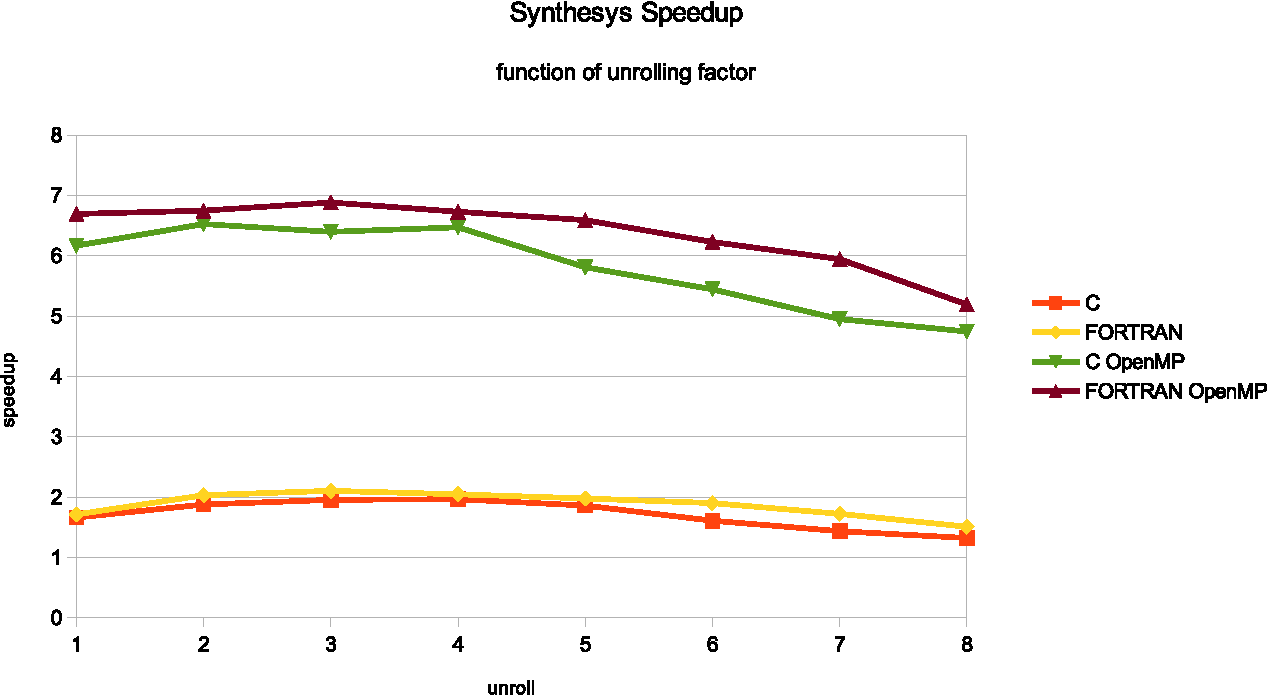
\includegraphics[scale=0.40]{Res_synthesis}
  \end{center}

  \begin{itemize}
    \item Reference is hand tuned code on target architecture
    \item Toward a BLAS-like library fo wavelets
  \end{itemize}
\end{frame}

\begin{frame}
  \frametitle{Real Applications: SPECFEM3D}

  \begin{itemize}
    \item SPECFEM3D ported to OpenCL using BOAST
    \begin{itemize}
      \item Unified code base (CUDA/OpenCL)
      \item Refactoring: kernel code base reduced by 40\%
      \item Similar performance on NVIDIA Hardware
      \item Non regression test for GPU kernels
    \end{itemize}
    \item On the Mont-Blanc prototype:
    \begin{itemize}
      \item OpenCL+MPI runs
      \item Speedup of 3 for the GPU version
    \end{itemize}
  \end{itemize}
\end{frame}

\section{Conclusions}

\begin{frame}
  \frametitle{Conclusions}
  \begin{itemize}
    \item BOAST v1.0 is released
    \item BOAST language features:
    \begin{itemize}
      \item Unified C and FORTRAN with OpenMP support,
      \item Unified OpenCL and CUDA support,
      \item Support for vector programming.
    \end{itemize}
    \item BOAST runtime features:
    \begin{itemize}
      \item Generation of parametric kernels,
      \item Parametric compilation,
      \item Non-regression testing of kernels,
      \item Benchmarking capabilities (PAPI support)
    \end{itemize}
  \end{itemize}
\end{frame}

\begin{frame}
  \frametitle{Perspectives}
  \begin{itemize}
    \item Find and port new kernels to BOAST
    \item Couple BOAST with other tools:
    \begin{itemize}
      \item Parametric space pruners (speed up optimization),
      \item Binary analysis (guide optimization),
      \item Source to source transformation (improve optimization),
      \item Binary transformation (improve optimization).
    \end{itemize}
    \item Improve BOAST:
    \begin{itemize}
      \item Improve the eDSL to make it more intuitive,
      \item Better vector support,
      \item Gather feedback.
    \end{itemize}
  \end{itemize}
\end{frame}

\end{document}
